\documentclass[tikz,border=3pt]{standalone}
\usepackage[T1]{fontenc}
\usepackage{tgheros}
\usepackage{newtxmath}
\usetikzlibrary{arrows.meta}
\renewcommand{\familydefault}{\sfdefault}
\definecolor{ink}{HTML}{22303A}
\definecolor{history}{HTML}{9A562F}
\definecolor{decision}{HTML}{215F81}
\begin{document}
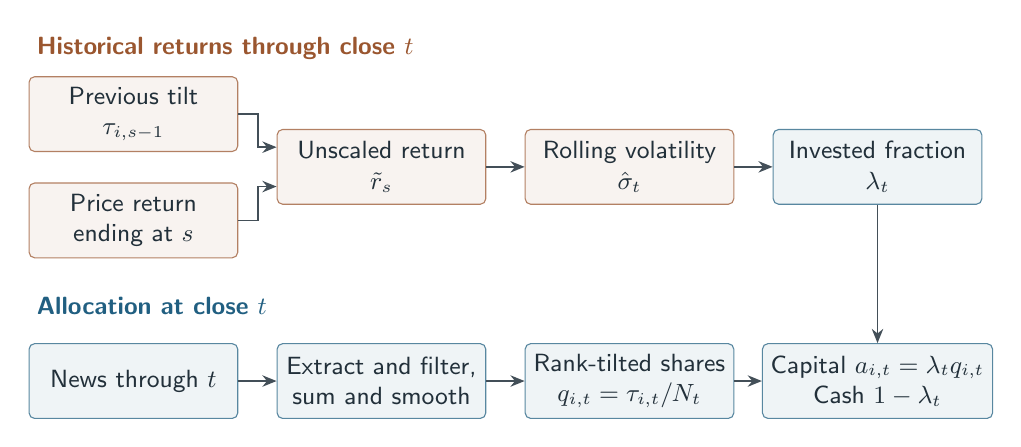
\begin{tikzpicture}[
  x=1cm,y=1cm,font=\sffamily\small,text=ink,
  box/.style={draw,rounded corners=2pt,align=center,inner sep=3pt,
    minimum width=2.65cm,minimum height=.95cm},
  past/.style={box,draw=history!75,fill=history!7},
  current/.style={box,draw=decision!75,fill=decision!7},
  flow/.style={-{Stealth[length=1.8mm,width=1.45mm]},draw=ink!85,line width=.65pt}
]
\node[anchor=west,text=history,font=\bfseries\small] at (-1.35,2.21)
  {Historical returns through close $t$};
\node[anchor=west,text=decision,font=\bfseries\small] at (-1.35,-1.07)
  {Allocation at close $t$};

\node[past] (tilt) at (0,1.37)
  {Previous tilt\\ $\tau_{i,s-1}$};
\node[past] (returns) at (0,.02)
  {Price return\\ ending at $s$};
\node[past] (unscaled) at (3.15,.70)
  {Unscaled return\\ $\tilde r_s$};
\node[past] (volatility) at (6.30,.70)
  {Rolling volatility\\ $\hat\sigma_t$};
\node[current] (budget) at (9.45,.70)
  {Invested fraction\\ $\lambda_t$};

\draw[flow] (tilt.east) -- ++(.25,0) |- ([yshift=2.5mm]unscaled.west);
\draw[flow] (returns.east) -- ++(.25,0) |- ([yshift=-2.5mm]unscaled.west);
\draw[flow] (unscaled) -- (volatility);
\draw[flow] (volatility) -- (budget);

\node[current] (news) at (0,-2.02)
  {News through $t$};
\node[current] (scores) at (3.15,-2.02)
  {Extract and filter,\\ sum and smooth};
\node[current] (allocation) at (6.30,-2.02)
  {Rank-tilted shares\\ $q_{i,t}=\tau_{i,t}/N_t$};
\node[current] (weights) at (9.45,-2.02)
  {Capital $a_{i,t}=\lambda_t q_{i,t}$\\ Cash $1-\lambda_t$};

\draw[flow] (news) -- (scores);
\draw[flow] (scores) -- (allocation);
\draw[flow] (allocation) -- (weights);
\draw[flow] (budget) -- (weights);
\end{tikzpicture}
\end{document}
